% !TEX root = ../thesis.tex
% !TEX spellcheck = en-US

\clearpage\section{Problem Definition: Multi-label Sentence Classification}
\label{sec:Problem Definition: Text Classification}

\subsection{Problem Formalism}
\label{subs:Problem Formalism}

Text classification, also known as text categorization, is the task of predicting a \emph{mapping} $\widetilde{\Phi} : \mathcal{D} \times \mathcal{C} \rightarrow \{True, False\}$ between a set of documents $\mathcal{D}$ and a set of classes or categories $\mathcal{C}$ using a model function $\Phi : \mathcal{D} \times \mathcal{C} \rightarrow \{True, False\}$. This means that were are trying to predict as good as possible the categories that each document belongs into, or vice versa the documents associated with each category. This mapping can thus be represented as a bipartite graph between the sets of documents $\mathcal{D}$ and categories $\mathcal{C}$ as shown in Figure~\ref{fig:bipartite-graph-text-classification}. In this representation vertices in the graph indicate a $True$ value in the mapping, indicating that the document and category are associated with each other, while missing vertices indicate that they are not ($False$).

\begin{wrapfigure}{r}{0.6\textwidth}
  \begin{center}
    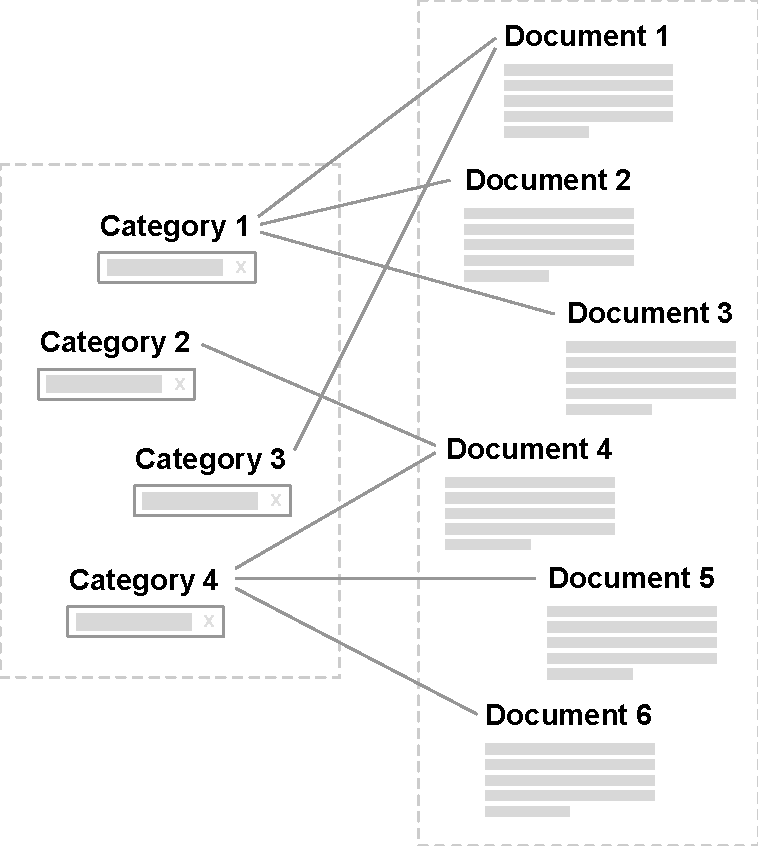
\includegraphics[width=0.6\textwidth]{img/bipartite-graph-text-classification}
  \end{center}
  \caption{Text classification visualized as a bipartite graph. Here the multi-label setting is shown where no additional constraints are enforced on the problem and hence each document can be assigned to multiple categories}
\label{fig:bipartite-graph-text-classification}
\end{wrapfigure}

Categories $\mathcal{C}$ are given as symbolic labels and documents $\mathcal{D}$ as chunks of text with variable length. We usually assume that no additional information such as metadata or other \emph{exogenous knowledge} is available on neither labels nor documents.
As~\cite{Sebastiani:2002aa} points out a consequence of relying solely on \emph{endogenous knowledge}, especially the semantics of a text, is that there is no objective ground truth to this task in most settings since semantics are a \emph{subjective} notion: \textquote{This is exemplified by the phenomenon of inter-indexer inconsistency [Cleverdon 1984]\todo{reference}: when two human experts decide whether to classify document $d_j$ under category $c_i$, they may disagree, and this in fact happens with relatively high frequency. A news article on Clinton attending Dizzy Gillespie’s funeral could be filed under Politics, or under Jazz, or under both, or even under neither, depending on the subjective judgment of the expert.}~\cite{Sebastiani:2002aa}

Additional constraints can be imposed on the problem to adapt it for different application scenarios. Firstly text classification can be either framed as \emph{single-label} classification where each document is assigned to only one single category or \emph{multi-label} classification where an assignment to several categories or also no category is possible. The multi-label case can also be formulated as $|\mathcal{C}|$ individual binary classification problems which of course assumes statistical independence between these prediction tasks.

In order to measure how successfully we are tackling the problem of text classification we need metrics that measure the effectiveness of our algorithm given a dataset. These will be discussed in Section~\ref{sub:Evaluation}.

\subsection{Dataset}
\label{subs:Dataset}
